% SC2005 Ch08 — File Systems, I/O, and Protection (no \documentclass)
\chapter{File Systems, I/O, and Protection}
\label{ch:filesec}

\begin{quote}
\emph{Files persist beyond processes; I/O connects computation to the world;
protection decides who may do what.} This chapter unifies storage management
with security.
\end{quote}

\noindent\textbf{Learning Outcomes.} After this chapter you will be able to:
\begin{enumerate}[label=(L\arabic*)]
  \item compare file allocation methods (contiguous, linked, FAT, indexed/inode);
  \item explain directory structures and journaling for crash consistency;
  \item describe disk scheduling (FCFS, SSTF, SCAN, C-SCAN, LOOK);
  \item outline I/O subsystem organization and buffering;
  \item reason about protection (ACLs vs.\ capabilities) and security threats.
\end{enumerate}

% ============================================================
\section{Files and Allocation}
\label{sec:files}

A \emph{file} is a named collection of bytes with attributes (name, size,
permissions, timestamps) stored in a directory entry. Allocation decides how
blocks are placed on disk:

\begin{itemize}
  \item \textbf{Contiguous:} file occupies consecutive blocks --- fast sequential
        access, but external fragmentation and resizing difficulty.
  \item \textbf{Linked:} blocks linked via pointers --- no fragmentation, but
        random access is $O(n)$ and pointers can be lost.
  \item \textbf{FAT (File Allocation Table):} linked allocation with a central
        table in memory --- supports random access via table walk; used in FAT32/exFAT.
  \item \textbf{Indexed (inode):} each file has an index block (inode) with
        direct, single-, double-, and triple-indirect pointers --- efficient
        for both small and large files (UNIX, ext4).
\end{itemize}

\begin{figure}[h!]
\centering
\begin{tikzpicture}[scale=0.74, every node/.style={font=\scriptsize},
  b/.style={draw, minimum width=1.0cm, minimum height=0.55cm, align=center}]
  % Inode diagram
  \node[draw, rounded corners, fill=blue!13, minimum width=2.0cm, minimum height=1.2cm, align=center] (inode) at (0,1.4) {Inode\\ \tiny direct[12]\\ single $\to$\\ double $\to$};
  \node[b, fill=green!13] (d0) at (3.0,2.2) {Data 0};
  \node[b, fill=green!13] (d1) at (4.4,2.2) {Data 1};
  \node[b, fill=orange!14] (ind1) at (3.0,1.1) {Indirect block};
  \node[b, fill=green!10] (dd0) at (4.6,1.1) {Data};
  \node[b, fill=green!10] (dd1) at (5.8,1.1) {Data};
  \node[b, fill=violet!12] (ind2) at (3.0,0.15) {Double-indirect};
  \node[b, fill=orange!10] (ind3) at (4.8,0.15) {Indirect};
  \draw[-{Stealth}, thick, blue!60!black] (inode) -- (d0);
  \draw[-{Stealth}, thick, blue!60!black] (inode) -- (d1);
  \draw[-{Stealth}, thick, orange!70!black] (inode) -- (ind1);
  \draw[-{Stealth}, thick] (ind1) -- (dd0); \draw[-{Stealth}, thick] (ind1) -- (dd1);
  \draw[-{Stealth}, thick, violet!70!black] (inode) -- (ind2);
  \draw[-{Stealth}, thick] (ind2) -- (ind3);
\end{tikzpicture}
\caption{UNIX inode: 12 direct pointers + single/double/triple indirect for large files.}
\label{fig:inode}
\end{figure}

\begin{figure}[h!]
\centering
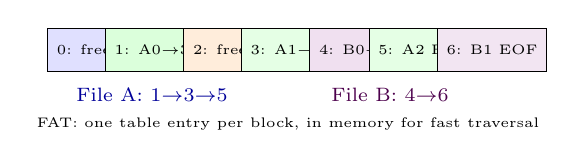
\begin{tikzpicture}[scale=0.72, every node/.style={font=\tiny},
  c/.style={draw, minimum width=0.9cm, minimum height=0.55cm, align=center}]
  \node[c, fill=blue!12] (a0) at (0,1.4) {0: free};
  \node[c, fill=green!14] (a1) at (1.2,1.4) {1: A0$\to$3};
  \node[c, fill=orange!14] (a2) at (2.4,1.4) {2: free};
  \node[c, fill=green!10] (a3) at (3.6,1.4) {3: A1$\to$5};
  \node[c, fill=violet!12] (a4) at (4.8,1.4) {4: B0$\to$6};
  \node[c, fill=green!10] (a5) at (6.0,1.4) {5: A2 EOF};
  \node[c, fill=violet!10] (a6) at (7.2,1.4) {6: B1 EOF};
  \node[font=\scriptsize, blue!60!black] at (1.2,0.6) {File A: 1$\to$3$\to$5};
  \node[font=\scriptsize, violet!60!black] at (5.4,0.6) {File B: 4$\to$6};
  \node[font=\tiny] at (3.6,0.1) {FAT: one table entry per block, in memory for fast traversal};
\end{tikzpicture}
\caption{FAT allocation: central table maps each block to next block or EOF.}
\label{fig:fat}
\end{figure}

\begin{example}[Inode capacity]
With 4\,KB blocks and 4-byte pointers, one indirect block holds $1024$ pointers.
12 direct $+$ single $+$ double indirect covers $12 + 1024 + 1024^2 \approx 10^6$
blocks $\approx 4$\,GB. Triple-indirect reaches terabytes.
\end{example}

\subsection{Directories and Journaling}
Directories map names $\to$ inodes (or FAT entries). Modern file systems use
\emph{journaling} (write-ahead log) to ensure crash consistency: metadata
changes are first written to a journal, then checkpointed. On crash, replay the
journal. Alternatives: copy-on-write (ZFS, btrfs) and soft updates.

Free-space management uses bitmaps ($1$ bit per block) or free lists.

% ============================================================
\section{Disk Scheduling and I/O}
\label{sec:disk-io}

Disk I/O time $=$ seek $+$ rotation $+$ transfer; seek dominates for HDDs.
Scheduling reorders the request queue:

\begin{itemize}
  \item \textbf{FCFS:} fair, no starvation, poor seek optimization.
  \item \textbf{SSTF:} nearest track first --- good throughput, starvation possible.
  \item \textbf{SCAN (elevator):} sweep arm back and forth, servicing along the way.
  \item \textbf{C-SCAN:} circular sweep (one direction only) for uniform wait.
  \item \textbf{LOOK / C-LOOK:} SCAN/C-SCAN but reverse at last request, not disk end.
\end{itemize}

For SSDs, seek is negligible; scheduling focuses on wear leveling and parallelism.

\begin{figure}[h!]
\centering
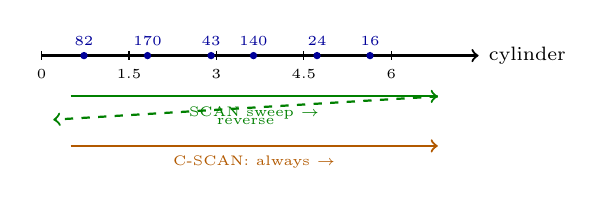
\begin{tikzpicture}[scale=0.74, every node/.style={font=\scriptsize}]
  \draw[->, thick] (0,0) -- (7.5,0) node[right]{cylinder};
  \foreach \x in {0,1.5,3,4.5,6} \draw[thin] (\x,0.08)--(\x,-0.08) node[below,font=\tiny]{\x};
  % requests as dots
  \foreach \x/\lbl in {0.8/82,2.0/170,3.2/43,4.0/140,5.2/24,6.2/16} {
    \fill[blue!60!black] (\x/1.1,0) circle (1.8pt) node[above,font=\tiny]{\lbl};
  }
  % SCAN path (schematic)
  \draw[->, thick, green!50!black] (0.5,-0.7) -- (6.8,-0.7) node[midway,below,font=\tiny]{SCAN sweep $\to$};
  \draw[->, thick, green!50!black, dashed] (6.8,-0.7) -- (0.2,-1.1) node[midway,below,font=\tiny]{reverse};
  \draw[->, thick, orange!70!black] (0.5,-1.55) -- (6.8,-1.55) node[midway,below,font=\tiny]{C-SCAN: always $\to$};
\end{tikzpicture}
\caption{Disk scheduling: request cylinders and SCAN vs.\ C-SCAN sweep direction (schematic).}
\label{fig:disk-sched}
\end{figure}

\begin{example}[SCAN vs.\ C-SCAN fairness]
SCAN gives edge cylinders shorter waits on the return sweep, biasing toward
recently visited tracks. C-SCAN wraps to the far end for near-uniform expected
wait, at the cost of one long seek. C-LOOK avoids seeking to the disk end.
\end{example}

\subsection{I/O Subsystem}
I/O is layered: application $\to$ kernel I/O subsystem (caching, spooling,
buffering) $\to$ device drivers $\to$ controllers (DMA, interrupts). Polling
wastes CPU; interrupt-driven I/O and DMA free the CPU during transfers.

% ============================================================
\begin{remark}[Buffering and caching]
The kernel buffers disk blocks in a page cache, coalesces writes, and
prefetches sequential reads. Double buffering overlaps computation with I/O:
while one buffer is processed, the next is filled by DMA.
\end{remark}

\section{Protection and Security}
\label{sec:protection}

\textbf{Protection} controls access of subjects (users/processes) to objects
(files, devices) via permissions. Two representations:

\begin{itemize}
  \item \textbf{ACL (Access Control List):} per object, list of (subject, rights).
  \item \textbf{Capability list:} per subject, list of (object, rights).
\end{itemize}
UNIX uses ACL-like mode bits (owner/group/other: rwx) plus extended ACLs.

\textbf{Security} defends against threats: malware, buffer overflows, privilege
escalation, and side channels. Principles: least privilege, defense in depth,
and complete mediation. Encryption at rest, authentication, and auditing
complement access control.

\begin{lstlisting}[language=C,caption={Checking UNIX permissions (sketch)}]
#include <sys/stat.h>
int can_read(const char *path, uid_t uid, gid_t gid){
    struct stat st; stat(path, &st);
    if(uid==st.st_uid) return st.st_mode & S_IRUSR;
    if(gid==st.st_gid) return st.st_mode & S_IRGRP;
    return st.st_mode & S_IROTH;
}
\end{lstlisting}

% ============================================================
% SSD scheduling differs fundamentally from HDD cylinder scheduling
\begin{remark}[SSD vs.\ HDD scheduling]
On SSDs, seek time is negligible and wear leveling plus internal parallelism
dominate. The OS focuses on TRIM/discard, write amplification, and queue depth
(NVMe) rather than cylinder ordering.
\end{remark}

\section{Exercises}
\label{sec:ch08-ex}
\begin{exercise}
For a 4\,KB block and 32-bit block pointers, how many blocks does a 12-direct
$+$ single $+$ double indirect inode address? What file size does that cover?
\end{exercise}
\begin{exercise}
Given disk queue $98,183,37,122,14,124,65,67$ with head at 53, compute total
seek distance for FCFS, SSTF, SCAN, and C-SCAN (disk 0--199, SCAN goes to end).
\end{exercise}
\begin{exercise}
Explain how journaling guarantees crash consistency. What is replayed after a
crash, and what is discarded?
\end{exercise}
\begin{exercise}
Compare ACLs vs.\ capabilities for revocation and least-privilege delegation.
Give an example where each shines.
\end{exercise}
\begin{exercise}
Why does SSD scheduling differ from HDD scheduling? What replaces seek
optimization as the primary concern?
\end{exercise}
